\documentclass[psamsfonts]{amsart}
\usepackage{amssymb,amsfonts}
\usepackage[all,arc]{xy}
\usepackage{enumerate}
\usepackage{mathrsfs}
\usepackage{tikz}
%\usepackage[letterpaper, portrait, margin=in]{geometry}
\usepackage{setspace}
\usepackage{graphicx}
\usepackage{caption}
\usepackage{subcaption}
\usepackage{breqn}
\usepackage{float}
%\onehalfspacing

%theoremstyle{plain} --- default
\newtheorem{thm}{Theorem}[section]
\newtheorem{cor}[thm]{Corollary}
\newtheorem{prop}[thm]{Proposition}
\newtheorem{lem}[thm]{Lemma}
\newtheorem{conj}[thm]{Conjecture}
\newtheorem{quest}[thm]{Question}

\theoremstyle{definition}
\newtheorem{defn}[thm]{Definition}
\newtheorem{defns}[thm]{Definitions}
\newtheorem{con}[thm]{Construction}
\newtheorem{exmp}[thm]{Example}


\newtheorem{exmps}[thm]{Examples}
\newtheorem{notn}[thm]{Notation}
\newtheorem{notns}[thm]{Notations}
\newtheorem{addm}[thm]{Addendum}
\newtheorem{exer}[thm]{Exercise}
\newtheorem{prob}[thm]{Problem}

\theoremstyle{remark}
\newtheorem{rem}[thm]{Remark}
\newtheorem{rems}[thm]{Remarks}
\newtheorem{warn}[thm]{Warning}
\newtheorem{sch}[thm]{Scholium}

\DeclareMathOperator{\sgn}{sgn}

%%%%COMMENT MACROS%%%%%%%%%%%%%%%%%%%%%%%%%%%%%%%%
%%%%COMMENT MACROS%%%%%%%%%%%%%%%%%%%%%%%%%%%%%%%%
%\usepackage{showlabels}
% LABELS!!
%\usepackage{times}%
%\usepackage[T1]{fontenc}%
%\usepackage{mathrsfs}%

%\usepackage[dvips]{graphics}
\usepackage{epsfig}
\usepackage{amsmath}
%\usepackage{hyperref, amsmath, amsthm, amsfonts, amscd, flafter,epsf}
%\usepackage{amsfonts,amsthm, ,amscd}
%\input amssym.def
%\input amssym.tex
\usepackage{color}
\newcommand{\will}[1]{{\color{blue} \sf $\clubsuit\clubsuit\clubsuit$ Will: [#1]}}
\newcommand{\artem}[1]{{\color{green} \sf $\spadesuit\spadesuit\spadesuit$ Artem: [#1]}}
%%%%%END  COMMENT MACROS(April 2011)%%%%%%%%%%%%%%%%%%%
%%%%%END  COMMENT MACROS(April 2011)%%%%%%%%%%%%%%%%%%%

\makeatletter
\let\c@equation\c@thm
\makeatother
\numberwithin{equation}{section}

\bibliographystyle{plain}

\title{Homework 1}

\author{A. Bolshakov}


\begin{document}

\maketitle


\begin{abstract}
My solutions. Code is at \texttt{https://github.com/atbolsh/RRR\_HW1}
\end{abstract}

\section{Problem 1}

Many constraint surfaces can be locally linearized. 
Let us examine the behavior of the dynamical system
\[
\dot{\mathbf{x}} = P_A(\mathbf{x}) - P_B(\mathbf{x})
\]
for this large class of systems by just looking at a simple, 2 dimensional case. 
Let constraint $A$ be
$x_2 = mx_1$
and constraing $B$ be 
$x_2 = -mx_1$
for some slope $m$.
(see Fig. \ref{fig1}).
%If our linear system has different slopes, we can easily get to this situation by rotating and dilating the coordinate axis.
%This is a linear map, so the dynamics are not affected by these transformations.


%Assume we start our dynamical system in the regime 
%$-mx_1 < x_2 < mx_1$ 
%(if this is not satisfied, we can easily rename the axes).


\begin{figure}
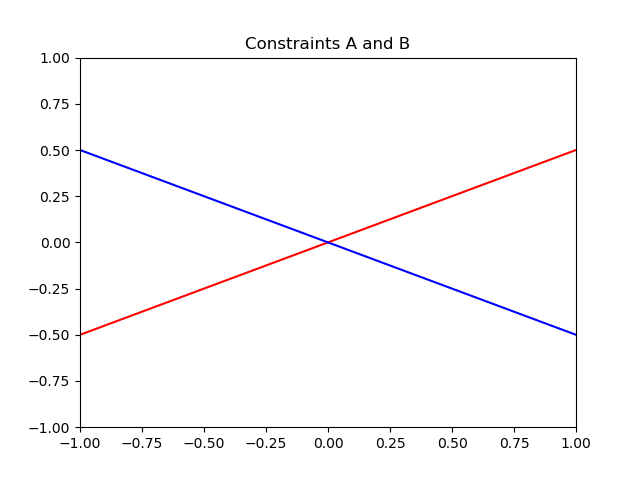
\includegraphics[scale=0.5]{Figure_1.png}
\caption{Example constraint surfaces. $A$ is red, $B$ is blue.}
\label{fig1}
\end{figure}



The system is simple enough that we can explicitly solve for $P_A$ and $P_B$:
\[
P_A \left( 
\begin{matrix}
x_1 \\ x_2
\end{matrix}
\right)
= 
\frac{1}{m^2 + 1}
\left(
\begin{matrix}
x_1 + mx_2 \\
mx_1 + m^2x_2
\end{matrix}
\right)
\]
\[
P_B \left( 
\begin{matrix}
x_1 \\ x_2
\end{matrix}
\right)
= 
\frac{1}{m^2 + 1}
\left(
\begin{matrix}
x_1 - mx_2 \\
m^2x_2 - mx_1
\end{matrix}
\right)
\]

We can ignore the $m^2 + 1$ coefficient as we only care about long term behavior.
So, we get
\[
\dot{\mathbf{x}} = 
P_A(\mathbf{x}) - P_B(\mathbf{x}) = 
\left(
\begin{matrix}
2mx_2 \\ 2mx_1
\end{matrix}
\right) 
= 
\left(
\begin{matrix}
0 & 2m \\
2m & 0
\end{matrix}
\right)
\mathbf{x}
\]


This is a classic linear hyperbolic system. The two eigenvalues are $\pm 2m$, so all trajectories except a set of measure $0$ will flow away.


\section{Problem 2}

\begin{figure}[H]
\centering
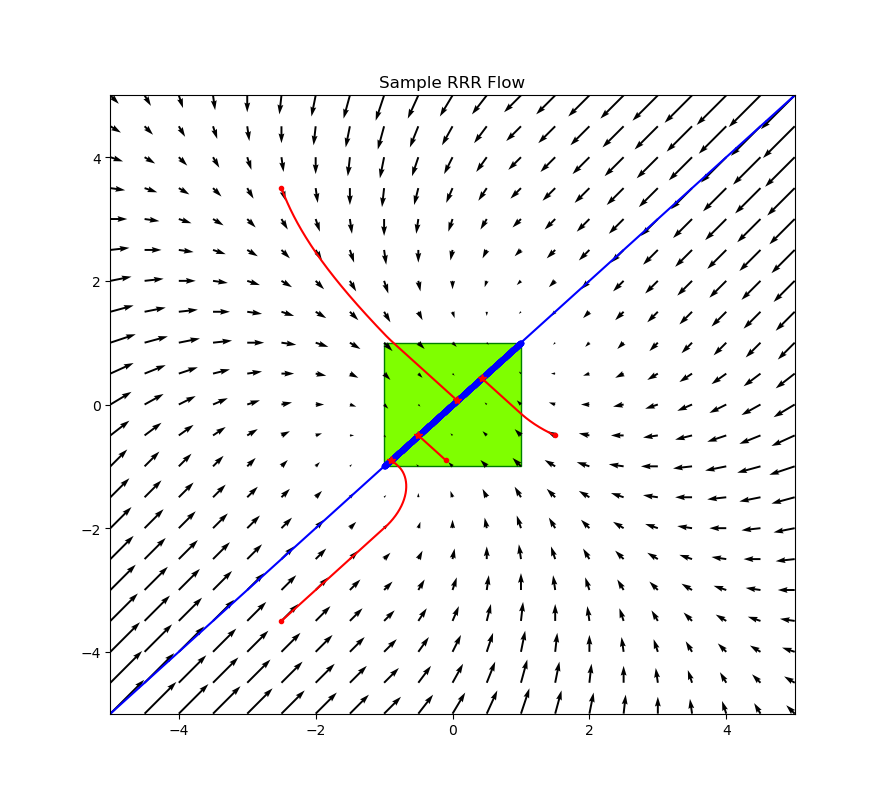
\includegraphics[width=\textwidth]{RRR_flow_final.png}
\caption{RRR flow, 
including constraint surfaces (blue and green), 
the set of fixed points (dark blue), 
4 sample trajectories (red), 
and the vector field for this dynamical system. 
Notice that since the problem domain $\mathbb{R}^2$ is spanned by the constraint surfaces, 
we do not need to worry about the distinction between $\mathbf{x}$ and $P_A(\mathbf{x})$.}
\label{fig2}
\end{figure}


Fig. \ref{fig2} shows the RRR flow. 
Numerical integration does not suggest any cycles, at least not in the smooth limit (I use $\beta = 0.01$); 
all $4$ of the tested trajectories converge, and my sample points represent all $4$ important regions:
\begin{enumerate}
\item
inside $A$; 
\item
directly above or to the left of $A$; 
\item
above-right /  below-left of $A$; 
\item
and above-left / below-right of $A$.
\end{enumerate}

It would be possible to go through and rigorously confirm that trajectories from all $4$ of these regions do, in fact, converge, 
but that= does not seem necessarry - after all, the entire point of the algorithms is to find solutions for problems where the 
flow is \textbf{not} fully understood.

\section{Problem 3}

Let $N$ be the length of our array (image), and let $P$ be the set of points $p \in \mathbb{R}^N$ such that 
$\text{sort}(p)$ gives the desired distribution (in our case, a uniform distribution).


Obviously, we wish to project some arbitrary point $x \in \mathbb{R}^N$ to this manifold $P$.
Denote by $p^{\star}$ the point with indeces in the same order as $x$.

Consider two candidate points $p, q \in P$ which differ only by a single permutation: 
for some $i \not= j$, $p_i = q_j$ and $p_j = q_i$, while for all $k \not= i, j$, $p_k = q_k$.

We have
\[
|q - x| - |p - x| = 
\]
\[
[(x_i - q_i)^2 + (x_j - q_j)^2] - [(x_i - p_i)^2 + (x_j - p_j)^2] = 
\]
\[
[(x_i - p_j)^2 + (x_j - p_i)^2] - [(x_i - p_i)^2 + (x_j - p_j)^2] = 
\]
\[
2x_ip_i + 2x_jp_j - 2x_ip_j - 2x_jp_i = 
\]
\[
2(x_i - x_j)(p_i - p_j)
\]

Now, if $x_i, x_j$ are in the same order as $p_i, p_j$ 
(either both $i$-indeces are smaller than the $j$s, or vice versa), 
this quantity is positive, so $p$ is closer to $x$ than $q$. If the order is mismatched, 
then $q$ is closer.

There are many sorting algorithms (for instance, \texttt{quickSort}) 
which are based on only exchanging values when they are in the wrong order. 
Therefore, starting at an arbitrary point $p_0 \in P$, it is possible 
to use any of these algorithms to construct a sequence $p_0, p_1, p_2, \ldots, p^{\star}$ with the property
\[
|p_{i + 1} - x| < |p_i - x|
\]

Therefore, $p^{\star}$ is closer to $x$ than any arbitrary point in $P$, as desired.

\[
\]

The flattened images are below; the python code is online in \texttt{prob3.py} 
(the code was written to be efficient, easy to read, and reusable.

\begin{figure}
\centering
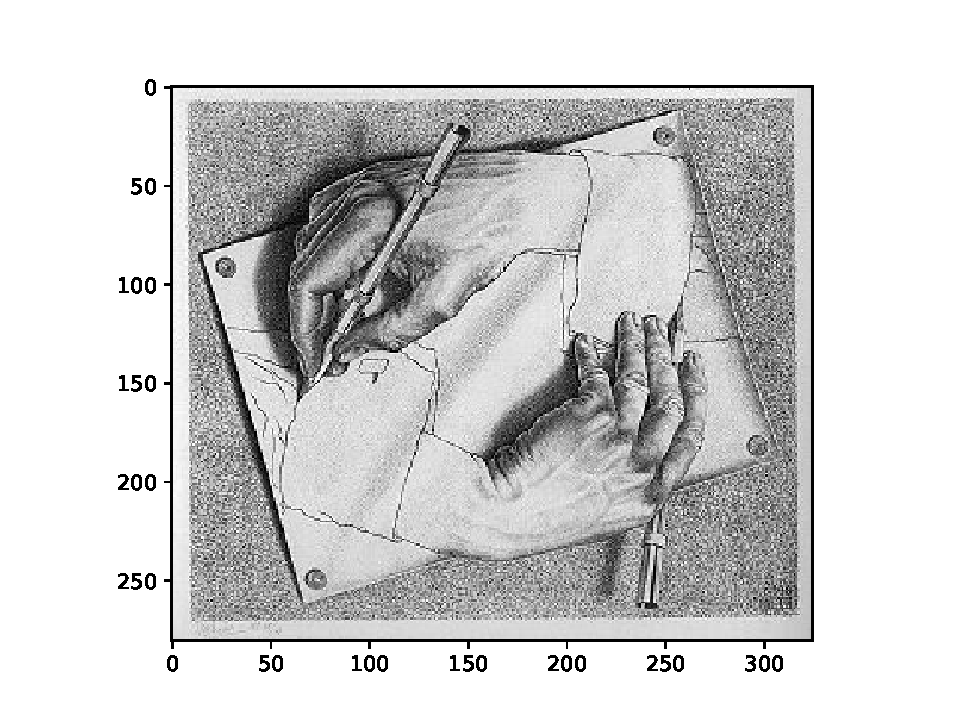
\includegraphics[width=\textwidth]{original.pdf}
\caption{Original Picture}
\label{fig3}
\end{figure}

\begin{figure}
\centering
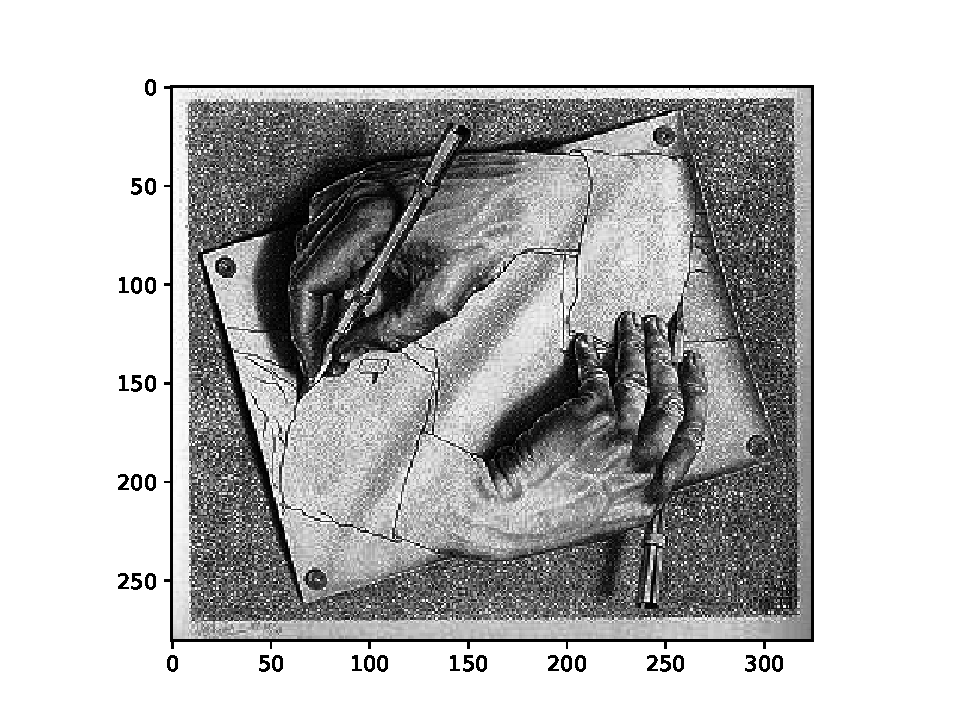
\includegraphics[width=\textwidth]{rescaled.pdf}
\caption{Output image with uniform distribution.}
\label{fig4}
\end{figure}

\begin{figure}
\centering
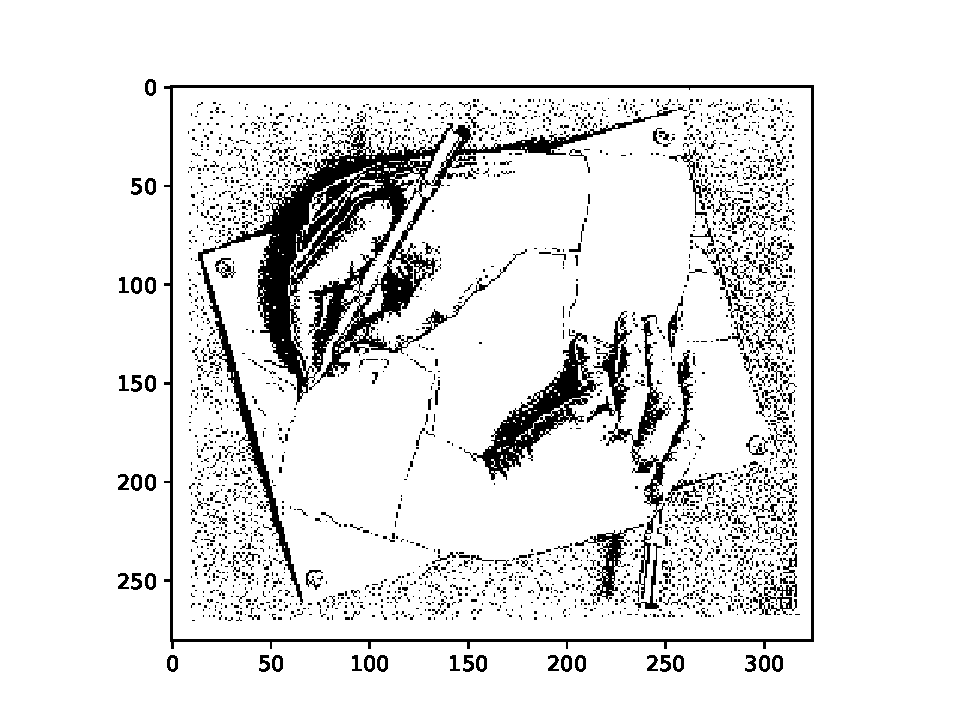
\includegraphics[width=\textwidth]{bimodal.pdf}
\caption{Projection onto a skewed bimodal distribution; 
the darkest $\frac{1}{6}$th pixels are black, the rest are white.}
\label{fig4}
\end{figure}


\end{document}

